% 4-page workshop draft. IEEE two-column conference format; switching to a CVPR or
% MICCAI/LNCS workshop template only changes the preamble.
% Every number in % generated by scripts/fidelity/paper_numbers.py -- do not edit
\newcommand{\NFrames}{12}
\newcommand{\NlabTotal}{2{,}958}
\newcommand{\NlabMin}{102}
\newcommand{\NlabMax}{362}
\newcommand{\NFits}{80}
\newcommand{\NPairs}{80}
\newcommand{\RecallLoG}{94\%}
\newcommand{\FramesLoG}{12}
\newcommand{\RecallWS}{89\%}
\newcommand{\FramesWS}{12}
\newcommand{\RecallCP}{75\%}
\newcommand{\FramesCP}{12}
\newcommand{\RecallCPthree}{82\%}
\newcommand{\FramesCPthree}{12}
\newcommand{\JXLmax}{82--120$\times$}
\newcommand{\JXLworst}{91\%}
\newcommand{\FarRatio}{319--603$\times$}
\newcommand{\JtkMaxRatio}{603$\times$}
\newcommand{\PairsNLoG}{80}
\newcommand{\PairsJLoG}{33}
\newcommand{\PairsLLoG}{14}
\newcommand{\ModNLoG}{38}
\newcommand{\ModJLoG}{4}
\newcommand{\ModLLoG}{10}
\newcommand{\ModDiffLoG}{$+$1.2}
\newcommand{\FarDiffLoG}{$-$16.8}
\newcommand{\FarJLoG}{29 of 42}
\newcommand{\FarJtkLoG}{98--103\%}
\newcommand{\FarLuxLoG}{25--107\%}
\newcommand{\PairsNWS}{80}
\newcommand{\PairsJWS}{63}
\newcommand{\PairsLWS}{0}
\newcommand{\ModNWS}{38}
\newcommand{\ModJWS}{22}
\newcommand{\ModLWS}{0}
\newcommand{\ModDiffWS}{$-$4.2}
\newcommand{\FarDiffWS}{$-$19.8}
\newcommand{\FarJWS}{41 of 42}
\newcommand{\FarJtkWS}{96--100\%}
\newcommand{\FarLuxWS}{32--98\%}
\newcommand{\PairsNCP}{80}
\newcommand{\PairsJCP}{56}
\newcommand{\PairsLCP}{0}
\newcommand{\ModNCP}{38}
\newcommand{\ModJCP}{22}
\newcommand{\ModLCP}{0}
\newcommand{\ModDiffCP}{$-$9.4}
\newcommand{\FarDiffCP}{$-$23.5}
\newcommand{\FarJCP}{34 of 42}
\newcommand{\FarJtkCP}{84--101\%}
\newcommand{\FarLuxCP}{27--91\%}
\newcommand{\PairsNCPthree}{78}
\newcommand{\PairsJCPthree}{28}
\newcommand{\PairsLCPthree}{14}
\newcommand{\ModNCPthree}{36}
\newcommand{\ModJCPthree}{2}
\newcommand{\ModLCPthree}{14}
\newcommand{\ModDiffCPthree}{$+$3.7}
\newcommand{\FarDiffCPthree}{$-$18.7}
\newcommand{\FarJCPthree}{26 of 42}
\newcommand{\FarJtkCPthree}{102--116\%}
\newcommand{\FarLuxCPthree}{29--118\%}
\newcommand{\PSNRjtkWins}{80 of 80}
\newcommand{\FrModPSNR}{$-$2.4}
\newcommand{\FrModPSNRCI}{$-$2.7 to $-$2.1}
\newcommand{\FrModPSNRPos}{0}
\newcommand{\FrModPSNRNeg}{12}
\newcommand{\FrFarPSNR}{$-$1.4}
\newcommand{\FrFarPSNRCI}{$-$1.6 to $-$1.3}
\newcommand{\FrFarPSNRPos}{0}
\newcommand{\FrFarPSNRNeg}{12}
\newcommand{\FrModLoG}{$+$1.3}
\newcommand{\FrModLoGCI}{$+$0.0 to $+$2.7}
\newcommand{\FrModLoGPos}{8}
\newcommand{\FrModLoGNeg}{4}
\newcommand{\FrModLoGP}{0.110}
\newcommand{\FrModLoGEOne}{$+$0.3}
\newcommand{\FrModLoGETwo}{$+$2.4}
\newcommand{\FrFarLoG}{$-$16.6}
\newcommand{\FrFarLoGCI}{$-$23.0 to $-$10.2}
\newcommand{\FrFarLoGPos}{1}
\newcommand{\FrFarLoGNeg}{11}
\newcommand{\FrFarLoGP}{0.004}
\newcommand{\FrFarLoGEOne}{$-$17.6}
\newcommand{\FrFarLoGETwo}{$-$15.5}
\newcommand{\FrModWS}{$-$4.0}
\newcommand{\FrModWSCI}{$-$5.3 to $-$2.7}
\newcommand{\FrModWSPos}{0}
\newcommand{\FrModWSNeg}{12}
\newcommand{\FrModWSP}{0.004}
\newcommand{\FrModWSEOne}{$-$2.1}
\newcommand{\FrModWSETwo}{$-$5.9}
\newcommand{\FrFarWS}{$-$19.3}
\newcommand{\FrFarWSCI}{$-$23.8 to $-$15.0}
\newcommand{\FrFarWSPos}{0}
\newcommand{\FrFarWSNeg}{12}
\newcommand{\FrFarWSP}{0.004}
\newcommand{\FrFarWSEOne}{$-$19.0}
\newcommand{\FrFarWSETwo}{$-$19.6}
\newcommand{\FrModCP}{$-$9.4}
\newcommand{\FrModCPCI}{$-$11.4 to $-$7.3}
\newcommand{\FrModCPPos}{0}
\newcommand{\FrModCPNeg}{12}
\newcommand{\FrModCPP}{0.004}
\newcommand{\FrModCPEOne}{$-$12.3}
\newcommand{\FrModCPETwo}{$-$6.5}
\newcommand{\FrFarCP}{$-$23.2}
\newcommand{\FrFarCPCI}{$-$28.0 to $-$18.3}
\newcommand{\FrFarCPPos}{0}
\newcommand{\FrFarCPNeg}{12}
\newcommand{\FrFarCPP}{0.004}
\newcommand{\FrFarCPEOne}{$-$29.0}
\newcommand{\FrFarCPETwo}{$-$17.5}
\newcommand{\FrModCPthree}{$+$3.5}
\newcommand{\FrModCPthreeCI}{$+$1.8 to $+$5.5}
\newcommand{\FrModCPthreePos}{10}
\newcommand{\FrModCPthreeNeg}{2}
\newcommand{\FrModCPthreeP}{0.010}
\newcommand{\FrModCPthreeEOne}{$+$1.0}
\newcommand{\FrModCPthreeETwo}{$+$6.1}
\newcommand{\FrFarCPthree}{$-$18.2}
\newcommand{\FrFarCPthreeCI}{$-$23.8 to $-$12.8}
\newcommand{\FrFarCPthreePos}{0}
\newcommand{\FrFarCPthreeNeg}{12}
\newcommand{\FrFarCPthreeP}{0.004}
\newcommand{\FrFarCPthreeEOne}{$-$20.3}
\newcommand{\FrFarCPthreeETwo}{$-$16.0}
\newcommand{\FrN}{12}
\newcommand{\FrFarNeg}{11--12}
\newcommand{\DPSNR}{1.0--6.8\,dB}
\newcommand{\EarlyAdvPts}{8--11}
\newcommand{\EarlyAdvRatio}{159--537$\times$}
\newcommand{\Kstar}{64{,}000}
\newcommand{\KstarCalFrames}{4}
\newcommand{\KstarFrames}{4}
\newcommand{\KstarRatio}{25--30$\times$}
\newcommand{\KstarLoG}{101--103\%}
\newcommand{\KstarWS}{96--100\%}
\newcommand{\KstarCP}{89--98\%}
\newcommand{\KstarCPthree}{102--105\%}
\newcommand{\KstarJtk}{99--102\%}
\newcommand{\GapWS}{$+$0 to $+$5}
\newcommand{\GapFramesWS}{10}
\newcommand{\LuxMidWS}{93--99\%}
\newcommand{\GapCP}{$+$4 to $+$15}
\newcommand{\GapFramesCP}{10}
\newcommand{\LuxMidCP}{82--94\%}
\newcommand{\GapCPthree}{$-$18 to $-$4}
\newcommand{\GapFramesCPthree}{10}
\newcommand{\LuxMidCPthree}{104--118\%}
\newcommand{\LuxMidLoG}{98--106\%}
\newcommand{\RuleGapBigWS}{1 of 12}
\newcommand{\RuleGapSmallWS}{11 of 12}
\newcommand{\RuleGapBigCPthree}{0 of 12}
\newcommand{\RuleGapSmallCPthree}{12 of 12}
\newcommand{\RuleGapBigCP}{11 of 12}
\newcommand{\RuleGapSmallCP}{1 of 12}
\newcommand{\RulePsnrOK}{4 of 8}
\newcommand{\CPwobble}{8}
\newcommand{\RepLoG}{2.1}
\newcommand{\RepWS}{3.5}
\newcommand{\RepCP}{3.7}
\newcommand{\CliffBelow}{2.5}
\newcommand{\CliffOne}{64--92\%}
\newcommand{\CrossRange}{1.1--3.1}
\newcommand{\LuxPSNRrange}{19.0--23.2\,dB}
\newcommand{\LuxPSNRspan}{2.6\,dB}
\newcommand{\FitA}{17--46\,min}
\newcommand{\FitH}{5--40\,min}
\newcommand{\SurvRho}{0.66}
\newcommand{\SurvN}{80}
 is generated from the result files by
% scripts/fidelity/paper_numbers.py -- do not edit numbers by hand.
\documentclass[conference]{IEEEtran}
\usepackage{graphicx}
\usepackage{booktabs}
\usepackage{amsmath}
\usepackage{xcolor}
\usepackage{siunitx}
\usepackage[hidelinks]{hyperref}
\newcommand{\pending}[1]{\textcolor{red}{#1}}   % waits on running jobs
\newcommand{\todo}[1]{\textcolor{orange}{[TODO: #1]}}
% generated by scripts/fidelity/paper_numbers.py -- do not edit
\newcommand{\NFrames}{12}
\newcommand{\NlabTotal}{2{,}958}
\newcommand{\NlabMin}{102}
\newcommand{\NlabMax}{362}
\newcommand{\NFits}{80}
\newcommand{\NPairs}{80}
\newcommand{\RecallLoG}{94\%}
\newcommand{\FramesLoG}{12}
\newcommand{\RecallWS}{89\%}
\newcommand{\FramesWS}{12}
\newcommand{\RecallCP}{75\%}
\newcommand{\FramesCP}{12}
\newcommand{\RecallCPthree}{82\%}
\newcommand{\FramesCPthree}{12}
\newcommand{\JXLmax}{82--120$\times$}
\newcommand{\JXLworst}{91\%}
\newcommand{\FarRatio}{319--603$\times$}
\newcommand{\JtkMaxRatio}{603$\times$}
\newcommand{\PairsNLoG}{80}
\newcommand{\PairsJLoG}{33}
\newcommand{\PairsLLoG}{14}
\newcommand{\ModNLoG}{38}
\newcommand{\ModJLoG}{4}
\newcommand{\ModLLoG}{10}
\newcommand{\ModDiffLoG}{$+$1.2}
\newcommand{\FarDiffLoG}{$-$16.8}
\newcommand{\FarJLoG}{29 of 42}
\newcommand{\FarJtkLoG}{98--103\%}
\newcommand{\FarLuxLoG}{25--107\%}
\newcommand{\PairsNWS}{80}
\newcommand{\PairsJWS}{63}
\newcommand{\PairsLWS}{0}
\newcommand{\ModNWS}{38}
\newcommand{\ModJWS}{22}
\newcommand{\ModLWS}{0}
\newcommand{\ModDiffWS}{$-$4.2}
\newcommand{\FarDiffWS}{$-$19.8}
\newcommand{\FarJWS}{41 of 42}
\newcommand{\FarJtkWS}{96--100\%}
\newcommand{\FarLuxWS}{32--98\%}
\newcommand{\PairsNCP}{80}
\newcommand{\PairsJCP}{56}
\newcommand{\PairsLCP}{0}
\newcommand{\ModNCP}{38}
\newcommand{\ModJCP}{22}
\newcommand{\ModLCP}{0}
\newcommand{\ModDiffCP}{$-$9.4}
\newcommand{\FarDiffCP}{$-$23.5}
\newcommand{\FarJCP}{34 of 42}
\newcommand{\FarJtkCP}{84--101\%}
\newcommand{\FarLuxCP}{27--91\%}
\newcommand{\PairsNCPthree}{78}
\newcommand{\PairsJCPthree}{28}
\newcommand{\PairsLCPthree}{14}
\newcommand{\ModNCPthree}{36}
\newcommand{\ModJCPthree}{2}
\newcommand{\ModLCPthree}{14}
\newcommand{\ModDiffCPthree}{$+$3.7}
\newcommand{\FarDiffCPthree}{$-$18.7}
\newcommand{\FarJCPthree}{26 of 42}
\newcommand{\FarJtkCPthree}{102--116\%}
\newcommand{\FarLuxCPthree}{29--118\%}
\newcommand{\PSNRjtkWins}{80 of 80}
\newcommand{\FrModPSNR}{$-$2.4}
\newcommand{\FrModPSNRCI}{$-$2.7 to $-$2.1}
\newcommand{\FrModPSNRPos}{0}
\newcommand{\FrModPSNRNeg}{12}
\newcommand{\FrFarPSNR}{$-$1.4}
\newcommand{\FrFarPSNRCI}{$-$1.6 to $-$1.3}
\newcommand{\FrFarPSNRPos}{0}
\newcommand{\FrFarPSNRNeg}{12}
\newcommand{\FrModLoG}{$+$1.3}
\newcommand{\FrModLoGCI}{$+$0.0 to $+$2.7}
\newcommand{\FrModLoGPos}{8}
\newcommand{\FrModLoGNeg}{4}
\newcommand{\FrModLoGP}{0.110}
\newcommand{\FrModLoGEOne}{$+$0.3}
\newcommand{\FrModLoGETwo}{$+$2.4}
\newcommand{\FrFarLoG}{$-$16.6}
\newcommand{\FrFarLoGCI}{$-$23.0 to $-$10.2}
\newcommand{\FrFarLoGPos}{1}
\newcommand{\FrFarLoGNeg}{11}
\newcommand{\FrFarLoGP}{0.004}
\newcommand{\FrFarLoGEOne}{$-$17.6}
\newcommand{\FrFarLoGETwo}{$-$15.5}
\newcommand{\FrModWS}{$-$4.0}
\newcommand{\FrModWSCI}{$-$5.3 to $-$2.7}
\newcommand{\FrModWSPos}{0}
\newcommand{\FrModWSNeg}{12}
\newcommand{\FrModWSP}{0.004}
\newcommand{\FrModWSEOne}{$-$2.1}
\newcommand{\FrModWSETwo}{$-$5.9}
\newcommand{\FrFarWS}{$-$19.3}
\newcommand{\FrFarWSCI}{$-$23.8 to $-$15.0}
\newcommand{\FrFarWSPos}{0}
\newcommand{\FrFarWSNeg}{12}
\newcommand{\FrFarWSP}{0.004}
\newcommand{\FrFarWSEOne}{$-$19.0}
\newcommand{\FrFarWSETwo}{$-$19.6}
\newcommand{\FrModCP}{$-$9.4}
\newcommand{\FrModCPCI}{$-$11.4 to $-$7.3}
\newcommand{\FrModCPPos}{0}
\newcommand{\FrModCPNeg}{12}
\newcommand{\FrModCPP}{0.004}
\newcommand{\FrModCPEOne}{$-$12.3}
\newcommand{\FrModCPETwo}{$-$6.5}
\newcommand{\FrFarCP}{$-$23.2}
\newcommand{\FrFarCPCI}{$-$28.0 to $-$18.3}
\newcommand{\FrFarCPPos}{0}
\newcommand{\FrFarCPNeg}{12}
\newcommand{\FrFarCPP}{0.004}
\newcommand{\FrFarCPEOne}{$-$29.0}
\newcommand{\FrFarCPETwo}{$-$17.5}
\newcommand{\FrModCPthree}{$+$3.5}
\newcommand{\FrModCPthreeCI}{$+$1.8 to $+$5.5}
\newcommand{\FrModCPthreePos}{10}
\newcommand{\FrModCPthreeNeg}{2}
\newcommand{\FrModCPthreeP}{0.010}
\newcommand{\FrModCPthreeEOne}{$+$1.0}
\newcommand{\FrModCPthreeETwo}{$+$6.1}
\newcommand{\FrFarCPthree}{$-$18.2}
\newcommand{\FrFarCPthreeCI}{$-$23.8 to $-$12.8}
\newcommand{\FrFarCPthreePos}{0}
\newcommand{\FrFarCPthreeNeg}{12}
\newcommand{\FrFarCPthreeP}{0.004}
\newcommand{\FrFarCPthreeEOne}{$-$20.3}
\newcommand{\FrFarCPthreeETwo}{$-$16.0}
\newcommand{\FrN}{12}
\newcommand{\FrFarNeg}{11--12}
\newcommand{\DPSNR}{1.0--6.8\,dB}
\newcommand{\EarlyAdvPts}{8--11}
\newcommand{\EarlyAdvRatio}{159--537$\times$}
\newcommand{\Kstar}{64{,}000}
\newcommand{\KstarCalFrames}{4}
\newcommand{\KstarFrames}{4}
\newcommand{\KstarRatio}{25--30$\times$}
\newcommand{\KstarLoG}{101--103\%}
\newcommand{\KstarWS}{96--100\%}
\newcommand{\KstarCP}{89--98\%}
\newcommand{\KstarCPthree}{102--105\%}
\newcommand{\KstarJtk}{99--102\%}
\newcommand{\GapWS}{$+$0 to $+$5}
\newcommand{\GapFramesWS}{10}
\newcommand{\LuxMidWS}{93--99\%}
\newcommand{\GapCP}{$+$4 to $+$15}
\newcommand{\GapFramesCP}{10}
\newcommand{\LuxMidCP}{82--94\%}
\newcommand{\GapCPthree}{$-$18 to $-$4}
\newcommand{\GapFramesCPthree}{10}
\newcommand{\LuxMidCPthree}{104--118\%}
\newcommand{\LuxMidLoG}{98--106\%}
\newcommand{\RuleGapBigWS}{1 of 12}
\newcommand{\RuleGapSmallWS}{11 of 12}
\newcommand{\RuleGapBigCPthree}{0 of 12}
\newcommand{\RuleGapSmallCPthree}{12 of 12}
\newcommand{\RuleGapBigCP}{11 of 12}
\newcommand{\RuleGapSmallCP}{1 of 12}
\newcommand{\RulePsnrOK}{4 of 8}
\newcommand{\CPwobble}{8}
\newcommand{\RepLoG}{2.1}
\newcommand{\RepWS}{3.5}
\newcommand{\RepCP}{3.7}
\newcommand{\CliffBelow}{2.5}
\newcommand{\CliffOne}{64--92\%}
\newcommand{\CrossRange}{1.1--3.1}
\newcommand{\LuxPSNRrange}{19.0--23.2\,dB}
\newcommand{\LuxPSNRspan}{2.6\,dB}
\newcommand{\FitA}{17--46\,min}
\newcommand{\FitH}{5--40\,min}
\newcommand{\SurvRho}{0.66}
\newcommand{\SurvN}{80}


\begin{document}

\title{Do Gaussian Splats Keep the Nuclei?\\An Object-Level Audit of Gaussian Volume Compression for Fluorescence Microscopy}

\author{\IEEEauthorblockN{\todo{author names}}
\IEEEauthorblockA{\todo{affiliation}}}

\maketitle

\begin{abstract}
Gaussian splats are being adopted to store and stream large 3D microscopy and medical
volumes, and their storage budgets are chosen and reported by PSNR. We ask the question
PSNR cannot answer: at a given number of bytes on disk, can standard analysis still find
the nuclei? On densely annotated \emph{C.~elegans} embryos (\NlabA{} and \NlabB{}
labelled nuclei), we compare a Gaussian-splat compressor (Luxar) with JPEG-XL, JPEG2000,
ZFP and downsampling at matched stored bytes, scoring two detectors against human labels.
JPEG-XL loses no nuclei up to its maximum compression (\JXLmax). Beyond
\SI{120}{\times}, splats are the best option tested (\LuxQuarterCP{} of nuclei kept at
$\approx$\SI{250}{\times} vs.\ \JtkQuarterCP{} for JPEG2000), but how many survive depends on
the detector: a blob detector keeps \LuxQuarterLoG{}, a learned segmenter
(Cellpose) keeps \LuxQuarterCP{}, and at \SIrange{55}{94}{\times} the segmenter already
loses \LuxMidLossCP{} of nuclei that JPEG-XL keeps. Loss collapses below
$\approx$3 splats per nucleus, while Luxar's PSNR stays within \LuxPSNRrange{} across
an \SI{18}{\times} range of budgets. A label-free survival check tracks the labelled result
(Spearman $\rho=\SurvRho$) and guards against the budget cliff, though not against
the segmenter's appearance gap.
\end{abstract}

\section{Introduction}
Light-sheet and confocal time-lapse microscopy produce terabytes per experiment, and
medical archives face the same pressure. Representing a volume as a set of anisotropic
3D Gaussians \cite{kerbl2023gaussian} is attractive for such data: the representation is
compact, continuous and renders directly on the GPU. Recent systems fit Gaussian splats
to microscopy volumes at scale \cite{royer2026luxar}, to slice-based microscopy and
ultrasound \cite{gaussianpile2026}, to medical volumes for compact storage
\cite{gstoken2026,martin2026fixedbudget}, and to tomographic reconstruction
\cite{li2025threedgr,zha2024r2gaussian}. Throughout, quality is measured by PSNR or SSIM,
and budgets are chosen by PSNR: Luxar selects its splat count by self-supervised held-out
PSNR \cite{batson2019noise2self} and explicitly describes its fits as intended for
visualisation rather than quantitative analysis \cite{royer2026luxar}.

What a microscopist needs from a compressed volume is that the analysis still works.
Whether a nucleus is still detectable is decided by a small, often faint, peak---exactly
the kind of structure an intensity-weighted fitting objective can trade away. Radiology
learned the same lesson for lossy codecs, where acceptability is judged by whether lesions
remain detectable, not by PSNR \cite{koff2006overview}. Gaussian volume compression has
not yet been held to that standard.

\textbf{Contributions.} (i)~A rate--detectability protocol for volumetric compression:
matched bytes on disk, dense human labels, two independent detectors, one-to-one matching
in physical units, and a faint/bright split. (ii)~Evidence on densely labelled
\emph{C.~elegans} embryos that JPEG-XL is safe up to its maximum ratio, that Gaussian splats
are the best option tested at higher ratios, and that their benefit depends on the
downstream detector while the codecs do not. (iii)~A budget cliff near 3 splats per
nucleus that PSNR does not reveal, and a label-free check that does.

\begin{figure*}[t]
\centering
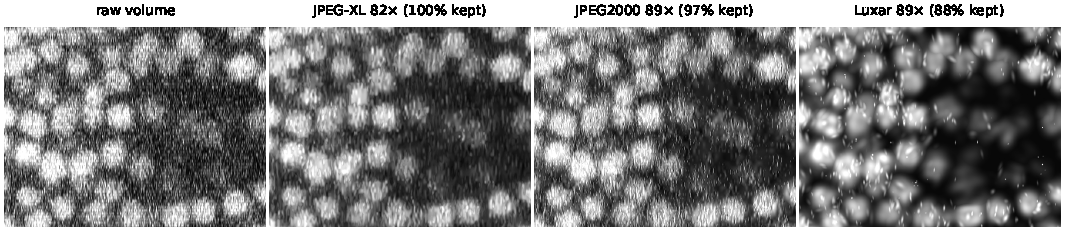
\includegraphics[width=\textwidth]{figures/fig_qualitative}
\caption{The same region of \emph{C.~elegans} t194 (3-slice maximum projection) from the raw
volume, JPEG-XL and Luxar at similar size. Titles give whole-frame nuclei kept by Cellpose.
JPEG-XL preserves the textured appearance of nuclei; Luxar renders smooth blobs on a black
background with thin streaks from elongated splats---an image distribution the learned
segmenter was not trained on, while a blob detector is unaffected.}
\label{fig:qual}
\end{figure*}

\section{Related Work}
Gaussian mixtures have long modelled nuclei for segmentation and lineage tracking
\cite{amat2014fast}; our question concerns Gaussians as a \emph{storage} format. Gaussian
splatting \cite{kerbl2023gaussian} has been adapted to CT \cite{zha2024r2gaussian,li2025threedgr},
to slice-to-volume MRI with closed-form point-spread functions
\cite{dannecker2026fast}, and to volume compression \cite{royer2026luxar,gaussianpile2026,
gstoken2026,martin2026fixedbudget}, each evaluated by image-fidelity metrics. Scientific
and image codecs---JPEG2000 \cite{taubman2002jpeg2000}, JPEG-XL \cite{alakuijala2019jpegxl},
and the error-bounded ZFP \cite{lindstrom2014fixed}---are the natural baselines at matched
size. Cell detection is benchmarked by the Cell Tracking Challenge \cite{ulman2017objective,
maska2023cell}; we use its labels and two standard detectors, a scale-normalised
Laplacian of Gaussian \cite{lindeberg1998feature} and Cellpose \cite{stringer2021cellpose}.

\section{Methods}
\textbf{Data.} Fluo-N3DH-CE from the Cell Tracking Challenge \cite{maska2023cell}:
\emph{C.~elegans} embryos, $35\times512\times708$ voxels of
$1.0\times0.09\times0.09\,\si{\micro\meter}$, 8-bit (\RawKiB{} per frame). Every nucleus
carries a tracking label; we use frames with \NlabA{} (t150) and \NlabB{} (t194) labelled
nuclei \pending{and a second embryo (sequence 02, t150/t180)}. Nuclei measure
\SI{3.6}{\micro\meter} across (median of the challenge's segmentation masks); all spatial
parameters below are fixed multiples of this diameter $D$.

\textbf{Compressors.} Luxar \cite{royer2026luxar} (default settings, 1000 iterations,
anisotropic voxel size, seeds $K\in\{10^3,\dots,6.4\times10^4\}$; stored size = its
\texttt{.gsplats.zarr} on disk). JPEG2000 (3D, OpenJPEG), JPEG-XL (per slice), ZFP
fixed-rate, and trilinear downsampling (stored as 16-bit). Each codec's quality
parameter is bisected to the byte size of each Luxar fit; rows that cannot reach the
target (JPEG-XL beyond \JXLmax, ZFP below 1~bit/voxel) are flagged.

\textbf{Detectors.} (a)~LoG: local maxima with a physically isotropic suppression window,
ranked by scale-normalised LoG response at $\sigma\in\{0.2,0.27,0.33,0.4\}D$; the top
$N$ are kept, with $N$ equal to the number of labelled nuclei, where recall equals
precision. (b)~Cellpose~3 \emph{nuclei} model \cite{stringer2021cellpose}, 2D per slice
stitched across $z$, diameter $D$, scored at its own operating point.

\textbf{Scoring.} Detections are matched one-to-one to labels within $r=0.6D$ by maximum
cardinality, then minimum distance; results at $0.4D$ and $0.8D$ are in
Table~\ref{tab:radius}. \emph{Nuclei kept} = nuclei found in the reconstruction / found in
the raw volume by the same detector (1.0 = nothing lost). Labelled nuclei are split into
faint and bright halves by their LoG response in the raw volume. \emph{Survival} is the
label-free fraction of the raw volume's 100 strongest LoG detections still found after
compression. Every reconstruction and detection is saved; code and results are
available \todo{repository link}.

\section{Results}
\begin{figure}[t]
\centering
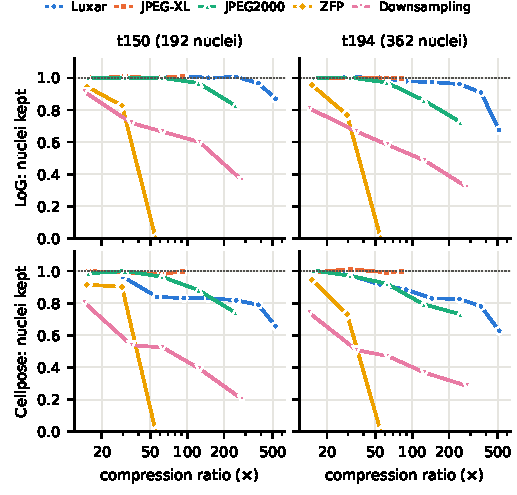
\includegraphics[width=\columnwidth]{figures/fig_rate_detectability}
\caption{Nuclei kept (relative to the raw volume) against compression ratio at matched
bytes on disk, for a blob detector (top) and Cellpose (bottom), on two \emph{C.~elegans}
frames. Luxar is blue. JPEG-XL cannot exceed \JXLmax{} on this data.}
\label{fig:rd}
\end{figure}

\textbf{Codecs.} JPEG-XL keeps every nucleus up to its maximum compression under both
detectors (Fig.~\ref{fig:rd}). JPEG2000 is nearly lossless for detection to
$\approx$\SI{60}{\times} and then loses faint nuclei first: at \SI{124}{\times} on t194
it loses \JtkFaintLoss{} faint but only \JtkBrightLoss{} bright nuclei (LoG).
Downsampling and fixed-rate ZFP fail early.

\textbf{Gaussian splats.} Beyond \SI{120}{\times}, Luxar is the best option tested: at
$\approx$\SI{250}{\times} it keeps \LuxQuarterLoG{} (LoG) and \LuxQuarterCP{} (Cellpose)
of nuclei, against \JtkQuarterLoG{} and \JtkQuarterCP{} for JPEG2000. Below
\SI{100}{\times}, its benefit depends on the detector. With the blob detector Luxar
matches the codecs; with Cellpose it keeps \LuxMidCP{} at \SIrange{55}{94}{\times}, where
JPEG-XL keeps \JXLMidCP{}. The Cellpose deficit is flat across a \SI{4}{\times} range of
splat budgets ($K$=4k--16k), so it reflects the appearance of splat reconstructions---smooth,
texture-free blobs with thin streak artefacts (Fig.~\ref{fig:qual}) that a learned
segmenter was not trained on---rather than a lack of capacity. The LoG detector responds most strongly to Gaussian blobs and thus flatters
splat reconstructions; the codecs are insensitive to the detector choice.

\begin{table}[t]
\centering
\caption{Nuclei kept (mean of two frames) near matched compression ratios, at match
radius $0.6D$. \pending{Sequence 02 to be added.}}
\label{tab:main}
\begin{tabular}{rrrrrrr}
\toprule
Ratio & Spl./nuc. & $\Delta$PSNR & LoG & Wshed & CP 2D & CP 3D \\
\midrule
$\approx$30$\times$ & 115--226 & $-$6.5 & +1.7$^{3}$ & $-$2.2$^{3}$ & $-$5.4$^{3}$ & +2.6$^{2}$ \\
$\approx$50$\times$ & 57--115 & $-$4.1 & +1.4$^{4}$ & $-$3.0$^{4}$ & $-$10.5$^{4}$ & +6.1$^{4}$ \\
$\approx$90$\times$ & 29--103 & $-$2.7 & +1.8$^{12}$ & $-$2.7$^{12}$ & $-$16.0$^{12}$ & +5.1$^{4}$ \\
$\approx$140$\times$ & 16--30 & $-$1.9 & $-$0.2$^{4}$ & $-$5.0$^{4}$ & $-$11.8$^{4}$ & +4.5$^{4}$ \\
$\approx$230$\times$ & 5--24 & $-$1.3 & +0.7$^{12}$ & $-$6.2$^{12}$ & $-$9.6$^{12}$ & +2.3$^{4}$ \\
$\approx$350$\times$ & 2--10 & $-$1.2 & $-$3.4$^{12}$ & $-$10.3$^{12}$ & $-$12.6$^{12}$ & $-$4.2$^{4}$ \\
$\approx$480$\times$ & 0.4--6.1 & $-$1.6 & $-$21.8$^{12}$ & \textbf{$-$22.9}$^{12}$ & $-$27.6$^{12}$ & \textbf{$-$26.5}$^{4}$ \\
\bottomrule
\end{tabular}

\end{table}

\textbf{The budget cliff.} Loss is abrupt once splats become scarce relative to nuclei
(Table~\ref{tab:cliff}): at one splat per nucleus Luxar keeps \CliffOneLoG{} (LoG) /
\CliffOneCP{} (Cellpose) of nuclei, recovering to \CliffSevenLoG{} / \CliffSevenCP{} at
$\approx$7 per nucleus. Over the same budgets Luxar's PSNR moves only within
\LuxPSNRrange{} (Fig.~\ref{fig:psnr}), and at ratios $\le$\SI{100}{\times} PSNR ranks
Luxar below both codecs although the blob detector finds the same nuclei. Across all reconstructions, PSNR
orders \PSNRwrong{} of pairs separated by more than \SI{1}{dB} in the wrong direction for
faint nuclei kept.

\begin{table}[t]
\centering
\caption{The budget cliff: Luxar fits by splats per labelled nucleus.}
\label{tab:cliff}
\setlength{\tabcolsep}{3pt}\small
\begin{tabular}{ccrrcccc}
\toprule
Frame & Splats & per nuc. & Ratio & PSNR & LoG & Cellpose & Surv. \\
\midrule
t150 & 324 & 1.7 & 530$\times$ & 19.6 & 0.87 & 0.66 & 0.92 \\
t150 & 1{,}050 & 5.5 & 382$\times$ & 19.9 & 0.97 & 0.79 & 1.00 \\
t150 & 2{,}550 & 13.3 & 252$\times$ & 20.0 & 1.01 & 0.82 & 0.99 \\
t150 & 10{,}837 & 56.4 & 94$\times$ & 20.3 & 1.01 & 0.83 & 1.00 \\
\midrule
t194 & 360 & 1.0 & 515$\times$ & 19.1 & 0.67 & 0.63 & 0.74 \\
t194 & 1{,}155 & 3.2 & 366$\times$ & 19.6 & 0.91 & 0.78 & 0.87 \\
t194 & 2{,}638 & 7.3 & 244$\times$ & 19.8 & 0.96 & 0.83 & 0.90 \\
t194 & 11{,}202 & 30.9 & 89$\times$ & 20.1 & 0.98 & 0.88 & 0.96 \\
\bottomrule
\end{tabular}

\end{table}

\begin{figure}[t]
\centering
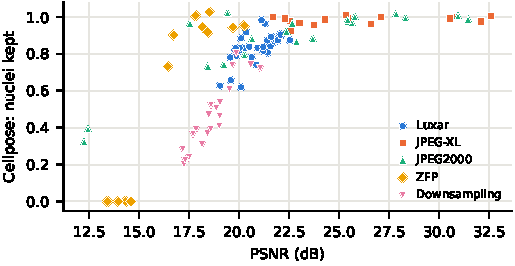
\includegraphics[width=\columnwidth]{figures/fig_psnr_blind}
\caption{PSNR against nuclei kept (Cellpose) for every reconstruction. Luxar's PSNR
barely changes while nuclei kept ranges from \CliffOneCP{} to near 1.}
\label{fig:psnr}
\end{figure}

\textbf{A label-free guard.} Survival, which needs no labels, tracks nuclei kept across
Luxar budgets (Spearman $\rho=\SurvRho$, $n=\SurvN$). Choosing the smallest budget with
survival $\ge0.95$ keeps \GuardKept{} of labelled nuclei: the check catches the
budget cliff but, being itself a blob-detector measure, not the appearance gap of learned
segmenters.
\pending{Luxar's own self-calibrated budget $K^\ast$ places at \ldots{} on this curve.}

\begin{table}[t]
\centering
\caption{Match-radius sensitivity: nuclei found in the raw volume and nuclei kept by
Luxar at $\approx$\SI{90}{\times} (t150).}
\label{tab:radius}
\begin{tabular}{lcccccc}
\toprule
 & \multicolumn{3}{c}{LoG} & \multicolumn{3}{c}{Cellpose (2D)} \\
\cmidrule(lr){2-4}\cmidrule(lr){5-7}
Radius & raw & JXL & Luxar & raw & JXL & Luxar \\
\midrule
0.4$D$ & 1009 & 1.00 & 1.02 & 658 & 1.01 & 0.84 \\
0.6$D$ & 1032 & 1.00 & 1.01 & 788 & 0.97 & 0.88 \\
0.8$D$ & 1034 & 1.00 & 1.01 & 796 & 0.99 & 0.90 \\
\bottomrule
\end{tabular}

\end{table}

\section{Discussion and Limitations}
Gaussian splats compress fluorescence volumes further than standard codecs while keeping
most nuclei detectable---but only above a budget that PSNR cannot identify, and with a
detector-dependent loss for learned segmenters that no image-fidelity metric exposes.
We therefore recommend (i)~JPEG-XL wherever its ratio suffices; (ii)~for higher ratios,
validating splat budgets with an object-level check such as survival, and (iii)~reporting
rate--detectability curves with the detector that will be used downstream.

Limitations: one dataset family \pending{(two embryos)}; Cellpose is used in its
2D-stitched mode; Luxar fitting takes \LuxFitMin{} per volume on one A100 GPU versus
seconds for the codecs; the faint/bright split is defined by one detector's response; and
we test a single Gaussian compressor with default settings. Retraining or fine-tuning
segmenters on splat reconstructions may close the appearance gap and is future work, as
is the same audit for small low-contrast lesions in CT.

\section{Conclusion}
Measured at matched bytes against human labels, Gaussian-splat compression is the
strongest option for nucleus detection at high ratios, yet its safety depends on the budget
and on the downstream detector---two things PSNR does not show. Object-level
rate--detectability evaluation should accompany Gaussian volume compression.

\bibliographystyle{IEEEtran}
\bibliography{refs}

\end{document}
